\documentclass[a4paper]{article}
\usepackage[utf8]{inputenc}

\usepackage{graphicx}
\usepackage[bf]{subfigure}
\usepackage[bf]{caption}
% Section titles in sans-serif:
\usepackage{sectsty}
\usepackage{abstract}
\allsectionsfont{\sffamily}

%\renewcommand{\abstractname}{\textsf{Abstract} xxxx}
\renewcommand{\abstractnamefont}{\bfseries\textsf}

\usepackage[usenames,dvipsnames]{color}
\definecolor{seagreen}{RGB}{46,139,87}
\definecolor{codebg}{RGB}{255,255,150}
\usepackage{listings}
\usepackage[colorlinks]{hyperref}
\usepackage{url}	

\hypersetup{%
  citecolor=blue,
  linkcolor=blue,
  urlcolor=blue,
}%



\lstset{
  extendedchars=\true,
  inputencoding=utf8,
  language=Matlab,
  %showstringspaces=false,
  formfeed=\newpage,
  tabsize=4,
  %commentstyle=\itshape,
  basicstyle=\ttfamily\scriptsize,
  %basicstyle={\small\fontfamily{fvm}\fontseries{m}\selectfont},
  commentstyle=\color{Apricot}\bfseries,
  %commentstyle=\color{red}\itshape,
  stringstyle=\color{red},
  identifierstyle=\color{PineGreen},
  showstringspaces=false,
  keywordstyle=\color{blue}\bfseries,
  moredelim=[il][\large\textbf]{\#\# },
  morekeywords={models,range},
  numbers=left,
  numbersep=2pt,
  numberstyle=\tiny,%\color{blue}\bfseries,
  backgroundcolor=\color{codebg},
  literate=%
  {ã}{{\~a}}1
  {â}{{\^a}}1
  {õ}{{\~o}}1
  {á}{{\'a}}1
  {ú}{{\'u}}1
  {í}{{\'i}}1
  {é}{{\'e}}1
  {Ç}{{\c{C}}}1
  {Õ}{{\~O}}1
  {Ê}{{\^E}}1
  {ó}{{\'o}}1
  {à}{{\`a}}1
  {Â}{{\^A}}1
  {ô}{{\^o}}1
  {ê}{{\^e}}1
  {ç}{{\c{c}}}1
}

\newcommand{\code}[2]{
 \vspace{1em}
 \subsubsection*{#1}
 \lstinputlisting{#2}
}

%%%%%%%%%%%%%%%%%%%%%%%%%%%%%%%%%%%%%%%%
% You have two versions of the macro
% \draftnote{My note}. The first version puts notes (e.g. My note in the example)
% into the margin of your document. The second formats the note as nothing. You
% 'comment out' the version of the macro you don't want (using a % at the
% beginning of the line).
\newcommand{\draftnote}[1]{\marginpar{\tiny\raggedright\textsf{\hspace{0pt}#1}}}
%\newcommand{\draftnote}[1]{}

% This one is just for the comments for in-line text.
\newcommand{\indraftnote}[1]{\textcolor[HTML]{114406}{\texttt{\footnotesize[#1]}}}
%\newcommand{\indraftnote}[1]{}
\newcommand{\todo}[1]{\indraftnote{todo: #1}}
\newcommand{\ie}{{\it i.e.}}
\newcommand{\etc}{{\it etc}}
\newcommand{\eg}{{\it e.g.}}
\newcommand{\wrt}{{\it w.r.t. }}
\newcommand{\etal}{{\it et.\ al.\ }}
\newcommand{\etalf}{{\it et.\ al.}}


\begin{document}

\title{\textsf{Computer Vision Lab \#1\\ Pointwise Image Processing}
\marginpar{\vspace{-1.2cm}
\includegraphics[height=1.4cm] {figs/logo_uerj_cor_small.png}}} 

\author{Prof.\ Ricardo Fabbri, Ph.D.\footnote{Based on Image Understanding
2011 lab material from Ben Kimia, Brown University}\\[1em]
Polytechnic Institute at the Rio de Janeiro State University\\
\url{http://wiki.nosdigitais.teia.org.br/CV}
}
 

\date{\today}
\maketitle
\begin{abstract}
\noindent\begin{itemize}
\item Familiarize with the Scilab image
processing toolbox (SIP)~\cite{scilab,Fabbri:etal:Arxiv2012}.
\item Implement pointwise image processing operations such as thresholding,
sampling, quantization, and enhancements.
\end{itemize}
\end{abstract}
\vspace{2em}



The images you will need for the lab can be downloaded from the course
website.

\section{The Scilab Image Processing toolbox (SIP)}

\paragraph{Initial tasks:}
\begin{enumerate}
\item Install Scilab and SIP. You will need Linux or Mac OSX.
\item Go through the SIP demos and make sure you understand the \texttt{imshow, imread,
imwrite}, and the other commands showcased in the demo.
\begin{lstlisting}[numbers=none]
exec(SIPDEMO);
\end{lstlisting}
\item Read our paper about the toolbox and type in the commands~\cite{SIP}.
Make things work in the desired way even if they don't, since your version of
SIP and Scilab may be different.
\end{enumerate}

\section{Thresholding}

\begin{figure}
\centering
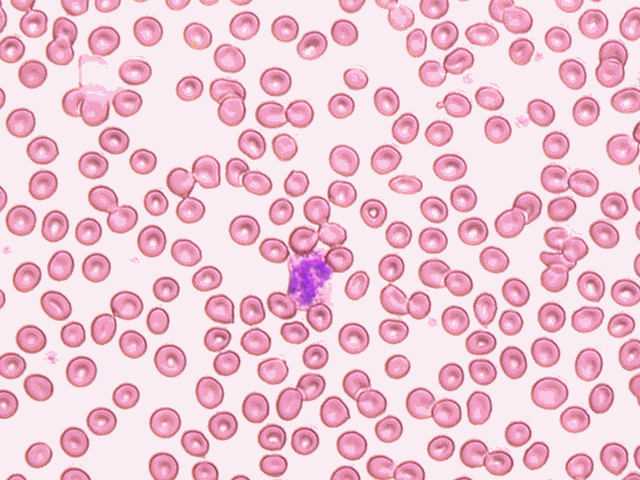
\includegraphics[width=0.5\linewidth]{figs/white_blood_cells.png}%
\caption{% 
White blood cells
}\label{fig:img1}
\end{figure}

\subsection{Basics} Using the white blood cell image~\ref{fig:img1} as seen below, threshold it to make any
non-cell area black. To do this, you will need to check each pixel in the image,
and if it is over $\tau_0$ (where $\tau_0$ is the threshold you have chosen) set the pixel’s
intensity to 0, otherwise, set to 1. You will need to play with $\tau_0$ to find its
optimal value. You will probably want to pass it into the function as a
parameter.
\code{Threshold code snippet}{threshold-code.sci}
\subsection{Bilevel Thresholding}
Using the snowman image~\ref{fig:img2}, perform bilevel thresholding. i.e. set all
pixels with intensity between $\tau_0$ and $\tau_1$ to 255 and set all pixels
less than $\tau_0$ 
to 0 and all pixels greater than $\tau_1$ to 0. The snowman is the region of interest,
you are thresholding for (where bob is, should be all white and the rest should
be black).

\begin{figure}
\centering
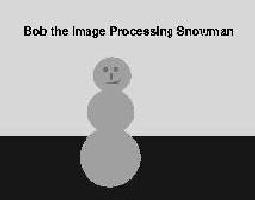
\includegraphics[width=0.5\linewidth]{figs/snowman.jpg}%
\caption{% 
Snowman image to practice thresholding. Notice \textsc{jpeg} compression artifacts as well.
}\label{fig:img2}
\end{figure}


\section{Contrast / Inversion}

\subsection{Brightness and Clipping} Increase the brightness of the image~\ref{fig:img3} by 10\% 
or decrease the brightness of the original by 10\% by adding/subtracting a value
$(I_0=25)$ from each pixel intensity. Try different values of $I_0$.

\begin{figure}
\centering
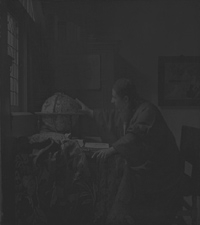
\includegraphics{figs/ImageA.jpg}%
\caption{% 
A poor contrast image
}\label{fig:img3}
\end{figure}

\paragraph{Hint:} Make sure you deal with values that fall outside the range of
the image (clipping).

\subsection{Color Image Inversion} Invert the white blood cell
image~\ref{fig:img1} in RGB. You should get something around the lines of
the sample in figure~\ref{fig:img4}
\paragraph{Hint:} Make sure pixel intensities are not negative
\begin{figure}
\centering
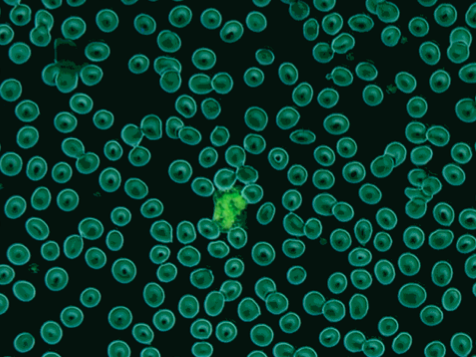
\includegraphics[trim=40mm 40mm 40mm 40mm, clip, width=0.5\linewidth]{figs/white_blood_cells-inverted.png}%
\caption{% 
Sample section of one possible color inversion of the image in figure~\ref{fig:img1}.
}\label{fig:img4}
\end{figure}



\section{Quantization: Reducing the number of colors}
The current cell image~\ref{fig:img1} has 256 possible values of pixel
intensity (but normalized from 0 to 1 \texttt{double} type in Scilab). 
Reduce
this to 8 levels (again normalized from 0 to 1). Make some observations about the quantization levels and image
quality. Do this by grouping intensity regions, \ie, set the intensity of all
pixels with current intensity between 0-31 to 16, between 32-63 to 48, 64-95 to
80,...etc.  How would you do this for 16 levels?

\section{Sub-Sampling}
Reduce the sampling of the white blood cells in image~\ref{fig:img1} by skipping
every other element.
\code{Sub-Sampling  code snippet}{sampling-code.sci}

\section{Playing with a Camera}

This lab will also give you a chance to become familiar with a digital video camera.
Use your own digital camera, smartphone, (or come by the visual computing and
computer graphics lab (room 110 at
\textsc{iprj/uerj}) to set up
a time to use the lab's digital video cameras such as the Sony PS3 Eye or 
an advanced surveillance camera) to take a few pictures or video clips, and upload them
to the computer. You will use this imagery for the next set of problems.

\subsection{Sensor noise}

\begin{enumerate}
\item Take at least 20 images (or a video with at least 20 frames) with your digital camera 
of the \textit{same} scene under the \textit{same}
illumination condition. Make sure \emph{nothing} changes in between taking these
images, so using a tripod a camera hooked up to your laptop is best.
\item Show the mean image and the standard deviation image. Scilab functions 
such as \texttt{mean()} and \texttt{std()} are available
\item Show the maximum difference from this mean image. How big is this? Does this depend
on the mean?
\item Pick one pixel across the 20 images, and plot the histogram,
\texttt{imhist()}. Discuss what the distribution of pixel intensity looks like.  \emph{Why does it
look like that?}
\item Repeat under a different lighting condition (light vs dark).
\end{enumerate}

\bibliography{personal}

\end{document}
